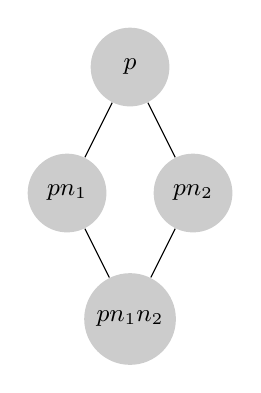
\begin{tikzpicture}
 [scale=.8,auto=center,every node/.style={circle,fill=black!20,font=\small,minimum size=1cm}]
  \node (p) at (4,10) {$p$};
  \node (n1) at (3,8)  {$p n_1$};
  \node (n2) at (5,8)  {$p n_2$};
  \node (n12) at (4,6)  {$p n_1 n_2$};


  \foreach \from/\to in {p/n1,p/n2,n1/n12,n2/n12}
    \draw (\from) -- (\to);
\end{tikzpicture}